\documentclass[10pt]{beamer}
\usepackage{../sty/acu-latex-thesis-talk}
\definecolor{Bluesky}{RGB}{0,128,255}
\title{Bayesian Textual Criticism since Hort}
\subtitle{A Synthesis and Demonstration\\\vspace{\baselineskip}2023 SBL Annual Meeting\\21 November 2023}
\author{Joey McCollum}
\institute{Australian Catholic University\\Institute for Religion and Critical Inquiry\\ \faEnvelope\quad\href{mailto:james.mccollum@myacu.edu.au}{james.mccollum@myacu.edu.au}\\ \faTwitter\ {\color{Bluesky}\faSquare}\quad @JoeyMcCollum\\ \faGithub\quad\href{https://github.com/jjmccollum}{jjmccollum}}
\date{} % insufficient space on this side, so move under subtitle
\begin{document}
	\begin{frame}
		\titlepage
	\end{frame}
	\section{Hort and the Stemmatic Model}
	\begin{frame}
		\begin{columns}
			\begin{column}{0.35\textwidth}
				\begin{center}
					\only<1>{
						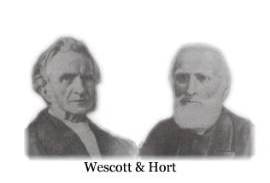
\includegraphics[width=\textwidth]{../img/westcott-hort-original.png}\\
						\footnotesize Source: Wikimedia Commons\\
						\phantom{(with adaptations)}
					}
					\only<2>{
						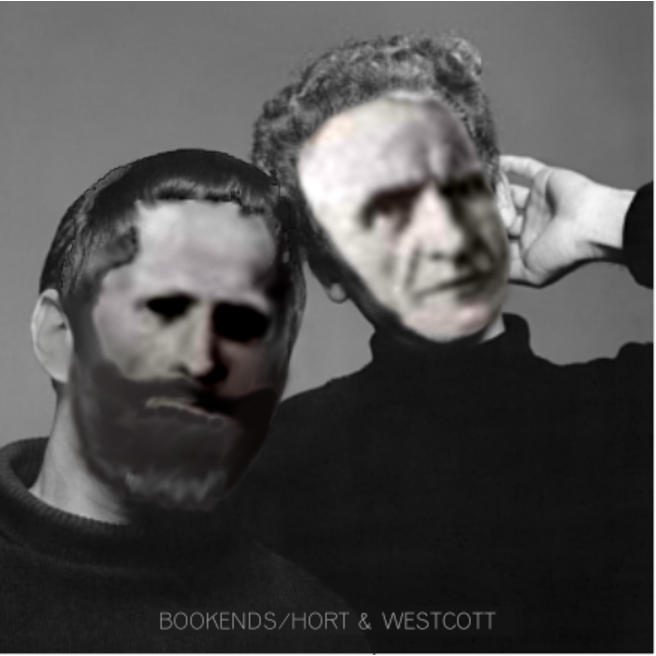
\includegraphics[width=0.675\textwidth]{../img/hort-westcott-bookends.pdf}\\
						\footnotesize Source: Wikimedia Commons\\
						(with adaptations)
					}
				\end{center}
				\vspace{0.5\baselineskip}
				\begin{itemize}
					\item Red, dotted = \emph{intrinsic probability}
					\item Green, dashed = \emph{transcriptional probability}
					\item Blue, solid = \emph{genealogical evidence}
				\end{itemize}
			\end{column}
			\begin{column}{0.65\textwidth}
				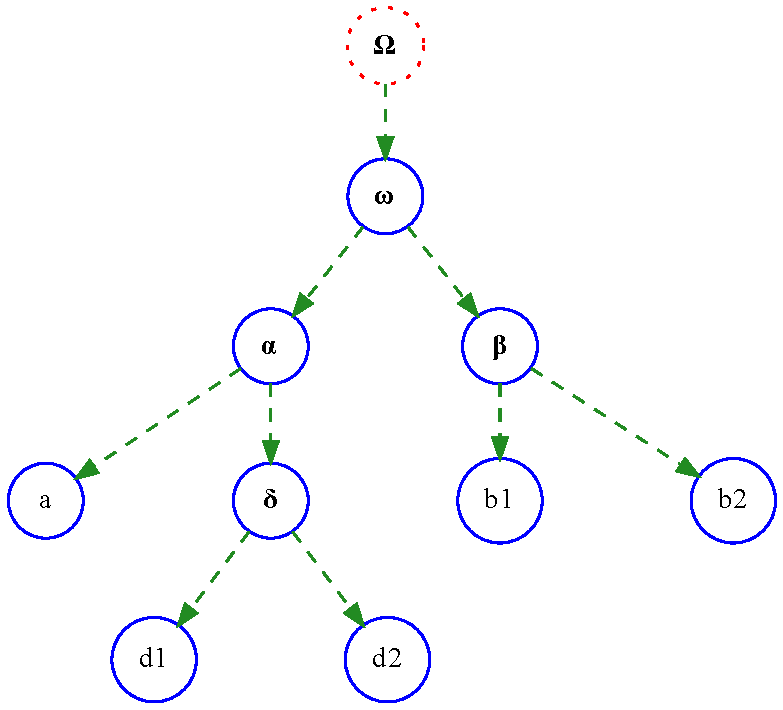
\includegraphics[width=\textwidth]{../img/stemma-evidence-overlay.pdf}
			\end{column}
		\end{columns}
	\end{frame}
	\section{Intrinsic Probability}
	\begin{frame}
		\begin{itemize}
			\item Similar to the rating system used in the UBS Commentary
		\end{itemize}
		\vspace{0.5\baselineskip}
		\begin{tabular}{p{0.25\textwidth} p{0.7\textwidth}}
			\emph{Rating} & \emph{Description}\\
			\hline
			\Rdg{a} \RelativeRating{A} \Rdg{b} & Reading \Rdg{a} is \emph{absolutely more likely} than reading \Rdg{b}.\\
			\Rdg{a} \RelativeRating{B} \Rdg{b} & Reading \Rdg{a} is \emph{highly more likely} than reading \Rdg{b}.\\
			\Rdg{a} \RelativeRating{C} \Rdg{b} & Reading \Rdg{a} is \emph{more likely} than reading \Rdg{b}.\\
			\Rdg{a} \RelativeRating{D} \Rdg{b} & Reading \Rdg{a} is \emph{slightly more likely} than reading \Rdg{b}.\\
			\Rdg{a} \EqualRating{} \Rdg{b} & Readings \Rdg{a} and \Rdg{b} have equal probability.
		\end{tabular}
		\vspace{0.5\baselineskip}
		\begin{columns}[T]
			\begin{column}{0.55\textwidth}
				\begin{itemize}
					\item Odds ratios between one reading and the next most likely one
					\item e.g., \Rdg{b} \RelativeRating{D} \Rdg{c} \RelativeRating{A} \Rdg{a} \EqualRating{} \Rdg{d} (right)
					\item Example values: $A = 19$, $B = 4$, $C = 1.5$, and $D = 1.1$
				\end{itemize}
			\end{column}
			\begin{column}{0.4\textwidth}
				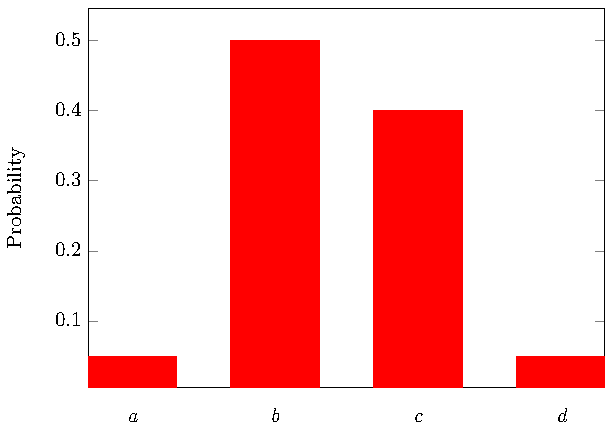
\includegraphics[width=\textwidth]{../img/intrinsic-probabilities-bar-chart.pdf}
			\end{column}
		\end{columns}
	\end{frame}
	\section{Transcriptional Probability}
	\begin{frame}
		\begin{itemize}
			\item A system of labels whose relative frequencies will be evaluated as part of the model
		\end{itemize}
		\begin{center}
			\begin{tabular}{p{0.25\textwidth} p{0.7\textwidth}}
					\emph{Tag} & \emph{Description}\\
					\hline
					\Clarification{} & Clarification in terms of grammar, style, or theology\\
					\AuralConfusion{} & Confusion of similar sounds (\textgreek{ι}/\textgreek{ει}/\textgreek{η}/\textgreek{οι}/\textgreek{υ}, \textgreek{αι}/\textgreek{ε}, \textgreek{ο}/\textgreek{ω}, \textgreek{β}/consonantal \textgreek{υ}, \textgreek{π}/\textgreek{φ}, \textgreek{κτλ}.)\\
					\LinguisticConfusion{} & Changes due to unfamiliarity with Greek grammar or changes to its rules over time\\
					\VisualError{} & Visual confusion of similar letters, skips and duplications of letters or words\\
					\Harmonization{} & Harmonization to parallel passage or near context\\
					\Byzantine{} & Assimilation to the dominant Byzantine text
			\end{tabular}
		\end{center}
		\begin{itemize}
			\item This allows us to model (and measure) different classes of scribal habits and a common type of mixture
		\end{itemize}
	\end{frame}
	\begin{frame}
		\begin{itemize}
			\item We can tag transitions between variant readings in a given unit according to their potential causes
			\item A stemma's probability is calculated along its branches in terms of transcriptional rates using \emph{Markov chains} (see below)
		\end{itemize}
		\begin{columns}[T]
			\begin{column}{0.5\textwidth}
				\footnotesize
				Eph 5:22\\
				\vspace{\baselineskip}
				\Rdg{a}: \textgreek{τοις ιδιοις ανδρασιν υποτασσεσθωσαν}\\
				\Rdg{b}: \textgreek{υποτασσεσθωσαν τοις ιδιοις ανδρασιν}\\
				\Rdg{c}: \textgreek{τοις ιδιοις ανδρασιν υποτασσεσθε}\\
				\Rdg{d}: \textgreek{υποτασσεσθε τοις ιδιοις ανδρασιν}\\
				\Rdg{e}: \textgreek{τοις ιδιοις ανδρασιν υποτασσομεναι}\\
				\Rdg{f}: \textgreek{τοις ιδιοις ανδρασιν} 
			\end{column}
			\begin{column}{0.5\textwidth}
				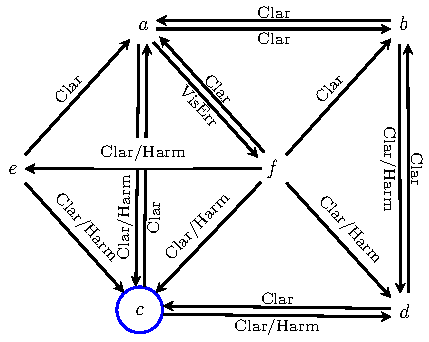
\includegraphics[scale=0.75]{../img/K5V22U6-12-transcriptional-probabilities.pdf}
			\end{column}
		\end{columns}
		\begin{itemize}
			\item Looks and functions like a local stemma, but is less constrained
		\end{itemize}
	\end{frame}
	\section{Genealogical Evidence}
	\begin{frame}
		\begin{itemize}
			\item Given a hypothesis $\mathcal{H}$ (i.e., a stemma with its parameters describing intrinsic probabilities, transcriptional probabilities, etc.) about how our collation data $\mathcal{D}$ arose, we can calculate its \emph{explanatory power} or \emph{likelihood} $\Pr(\mathcal{D} \mid \mathcal{H})$ using phylogenetic algorithms
			\item The \emph{posterior probability} $\Pr(\mathcal{H} \mid \mathcal{D})$ tells us how certain we can be about $\mathcal{H}$; we can estimate it by cleverly sampling different stemmata and combinations of parameters
		\end{itemize}
		\vspace{3\baselineskip}
		\begin{equation*}
			{\color{blue}\overbrace{\color{black}\Pr(\mathcal{H} \mid \mathcal{D})}^{\text{Posterior}}}
			= \frac{
			{\color{red}\overbrace{\color{black}\Pr(\mathcal{D} \mid \mathcal{H})}^{\text{Likelihood}}}
			{\color{green!50!black}\overbrace{\color{black}\Pr(\mathcal{H})}^{\text{Prior}}}
			}{
			{\color{orange}\underbrace{{\color{black}\Pr(\mathcal{D})}}_{\text{Probability of Data}}}
			}
		\end{equation*}
		\vspace{3.75\baselineskip}
	\end{frame}
	\section{Impact}
	\begin{frame}
		\only<1>{
			\begin{center}
				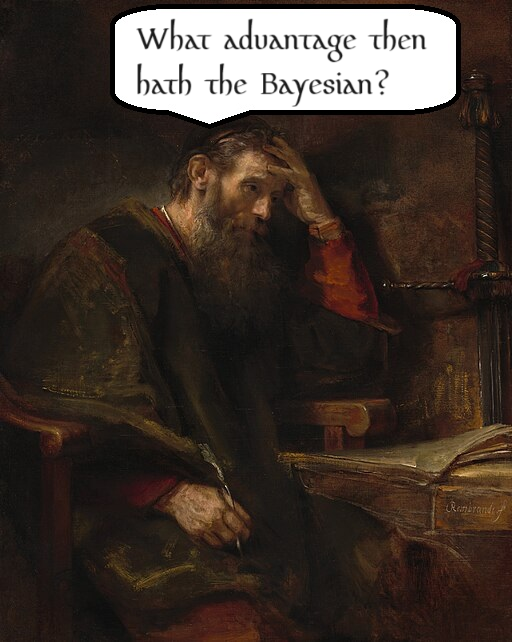
\includegraphics[scale=1]{../img/paul-comic.png}\\
				\footnotesize Source: Rembrandt van Rijn, \emph{The Apostle Paul} (Wikimedia Commons)\\
			\end{center}
		}
		\only<2->{
			\emph{Much in many ways!}
			\begin{itemize}
				\item<3-> A clean separation of concerns between different types of evidence
				\item<4-> Accommodation and resolution of tension between intrinsic and transcriptional evidence
				\item<5-> Built-in estimation of scribal habits
				\item<6-> Support for witness dates
				\item<7-> Inclusion of (sufficiently extant) versional and patristic sources
				\item<8-> A measure of (un)certainty about stemma branches, scribal habits, initial readings
				\item<9-> A set of candidate stemmata that can be reconciled to address contamination in a local-genealogical way
			\end{itemize}
		}
	\end{frame}
	\section{Demonstration}
	\subsection{1 Peter}
	\begin{frame}
		\begin{center}
			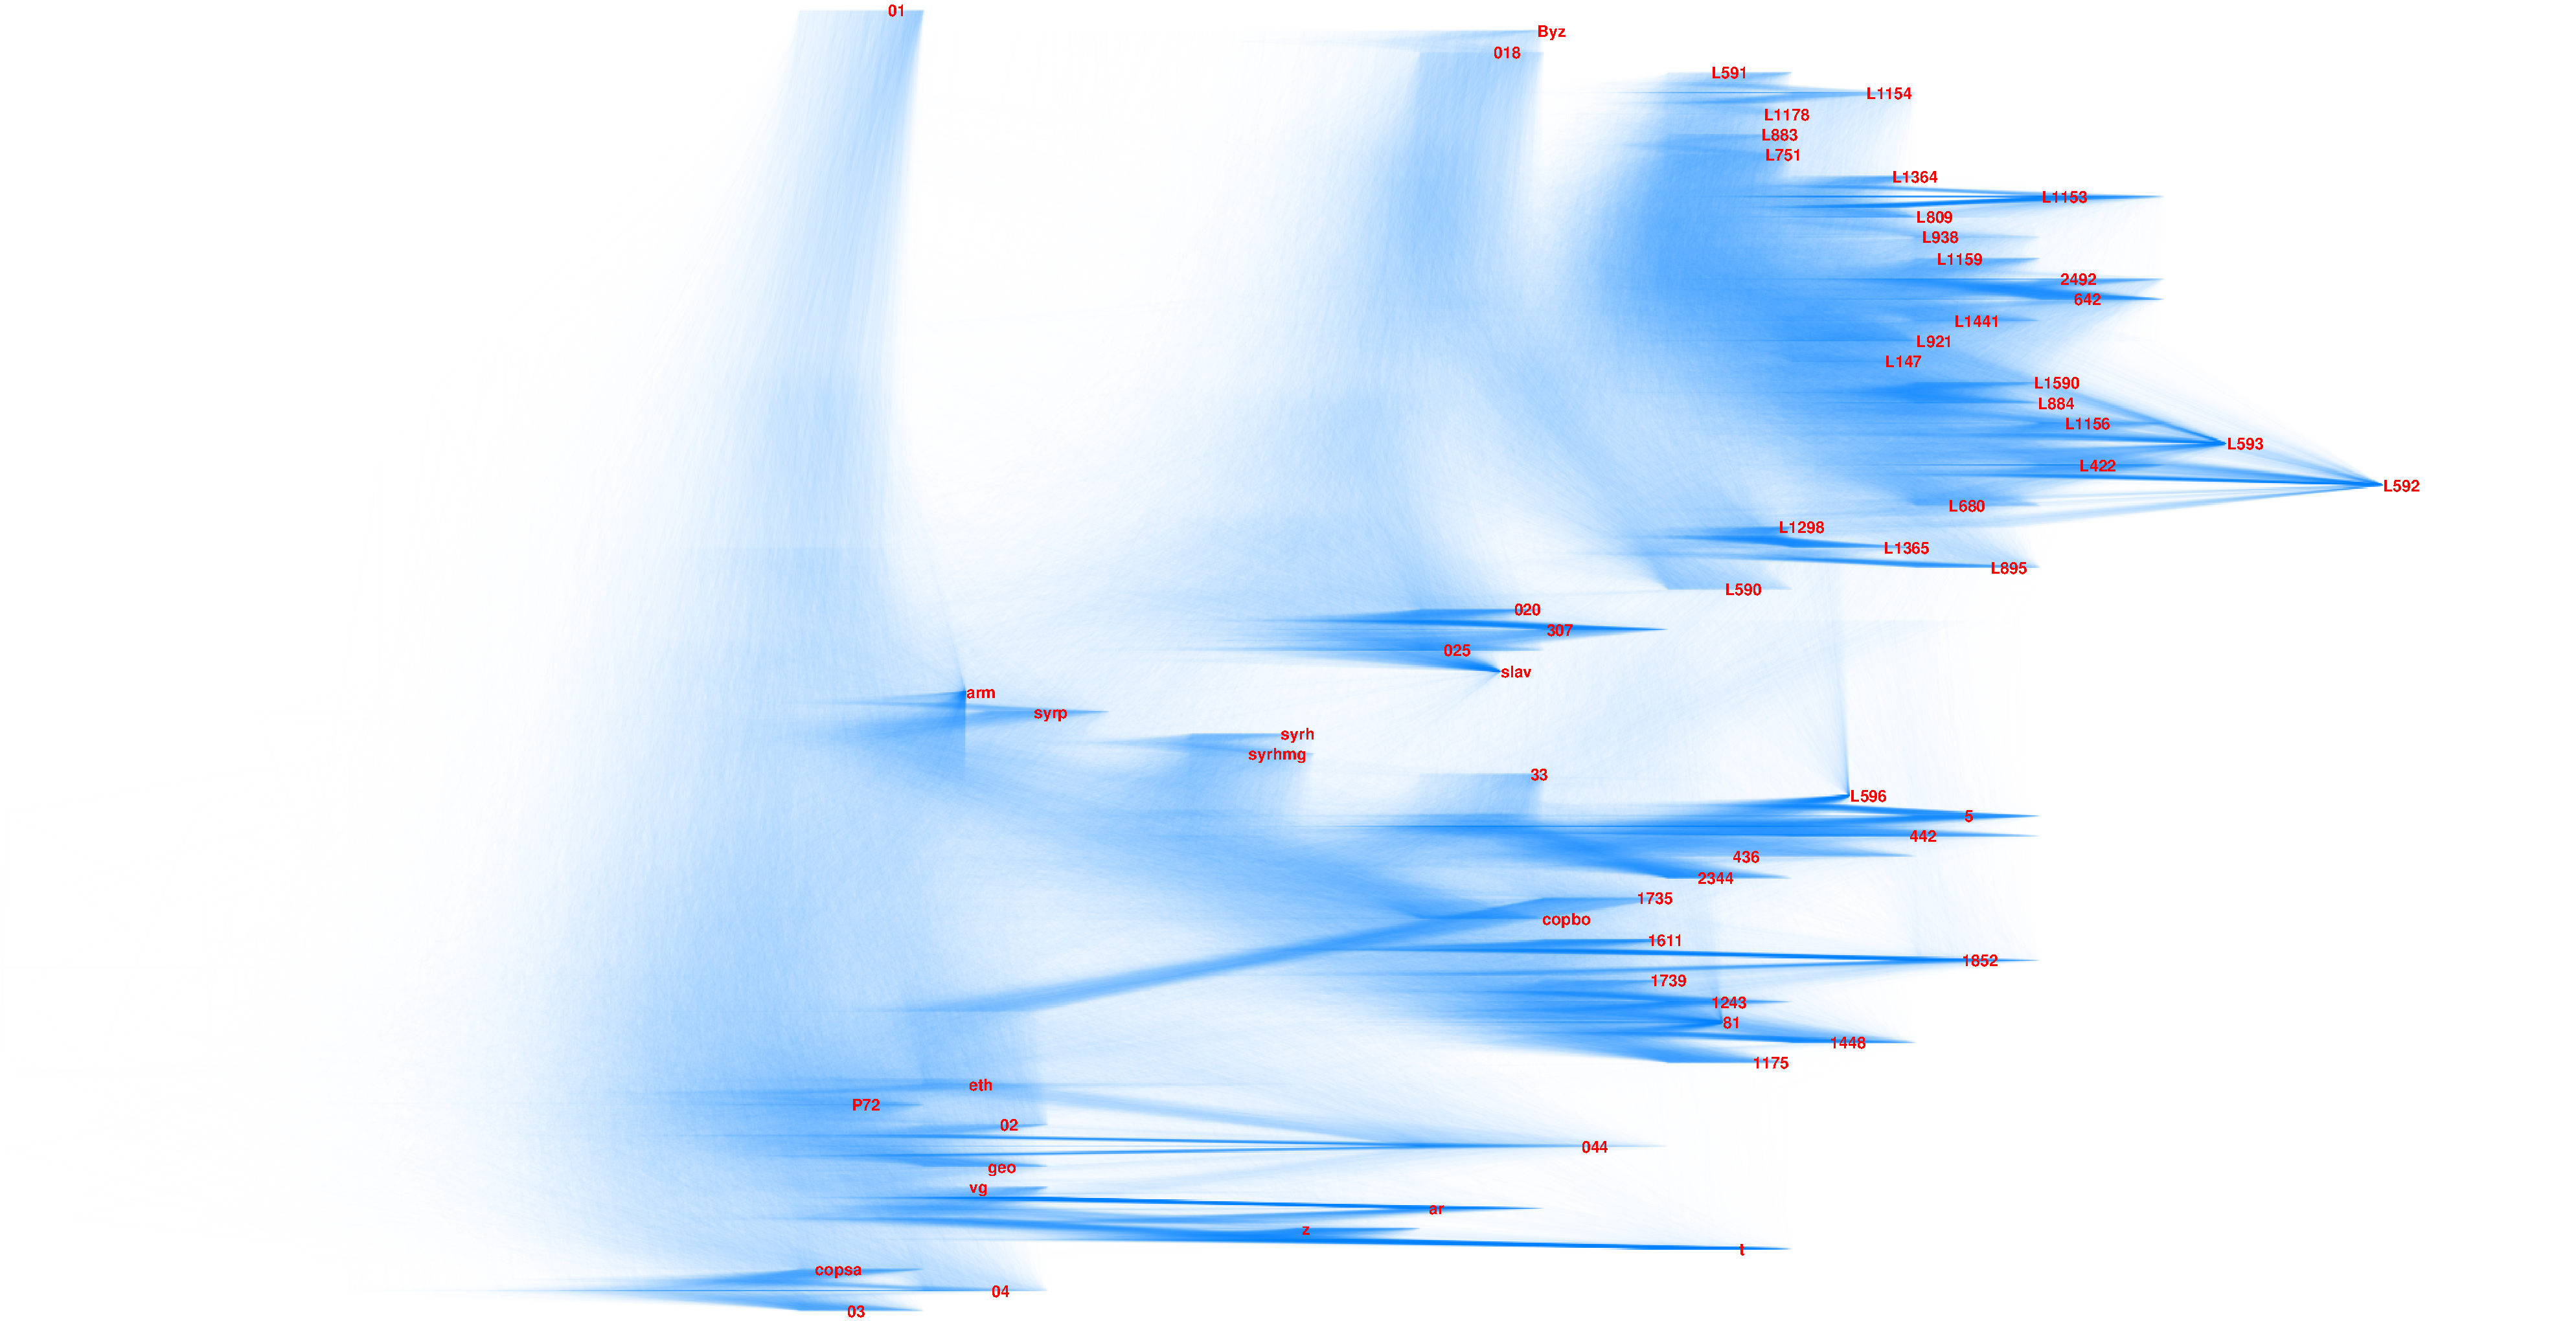
\includegraphics[width=\textwidth]{../img/ubs_1_peter_local_densitree.pdf}\\
			Posterior distribution of stemmata for subset of UBS 1 Peter data at UBS variation units (64 witnesses, 36 variation units, 20,000,000 iterations) with local clock model\\
		\end{center}
	\end{frame}
	\subsection{Revelation}
	\begin{frame}
		\begin{center}
			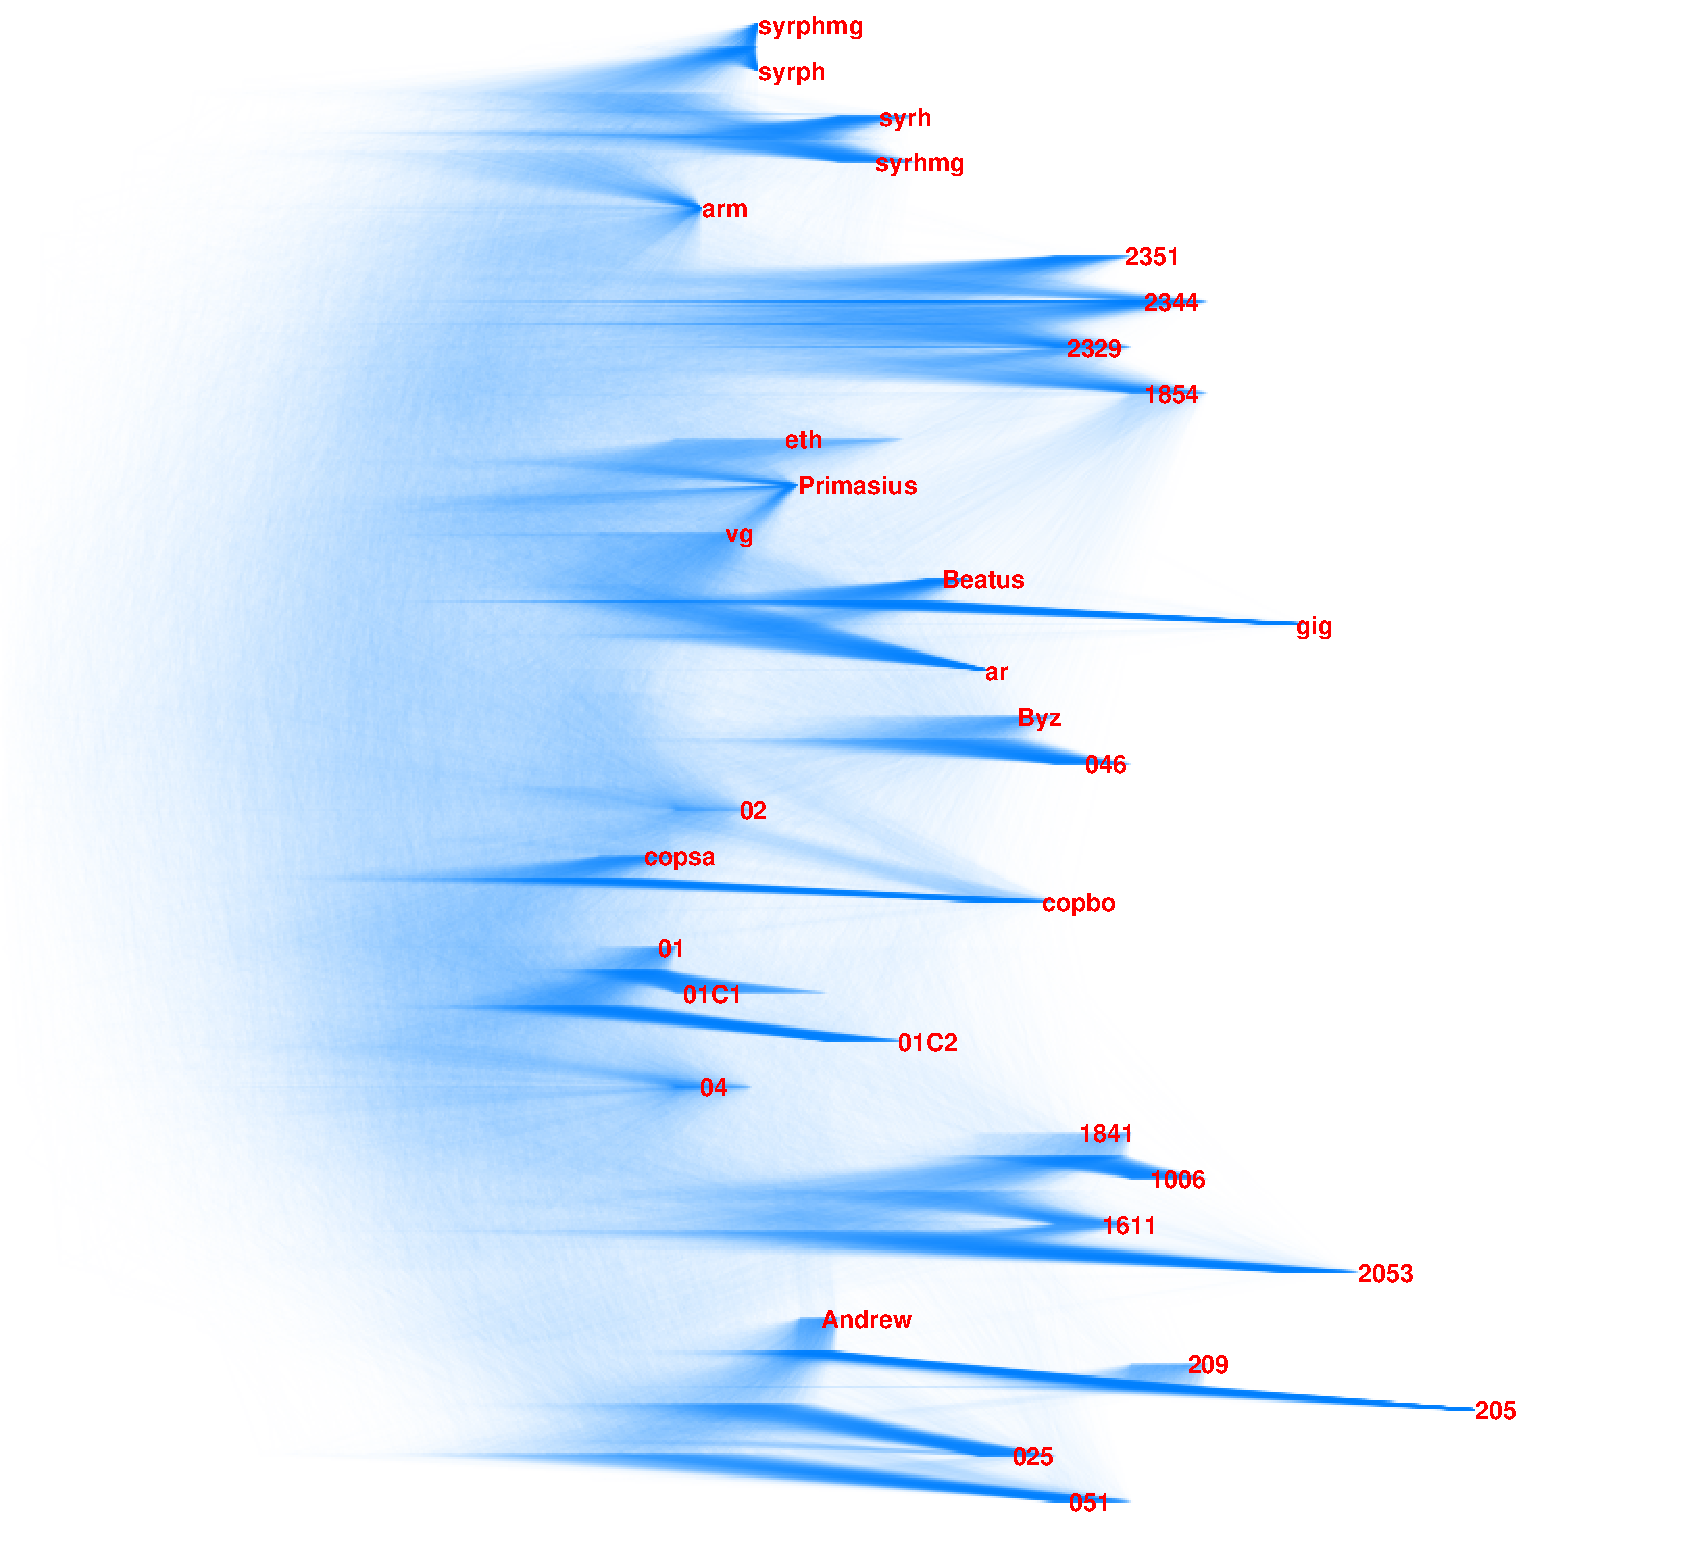
\includegraphics[width=0.6667\textwidth]{../img/ubs_revelation_local_densitree.pdf}\\
			Posterior distribution of stemmata for subset of UBS Revelation data at UBS variation units (33 witnesses, 70 variation units, 20,000,000 iterations) with local clock model\\
		\end{center}
	\end{frame}
	\begin{frame}
		\begin{center}
			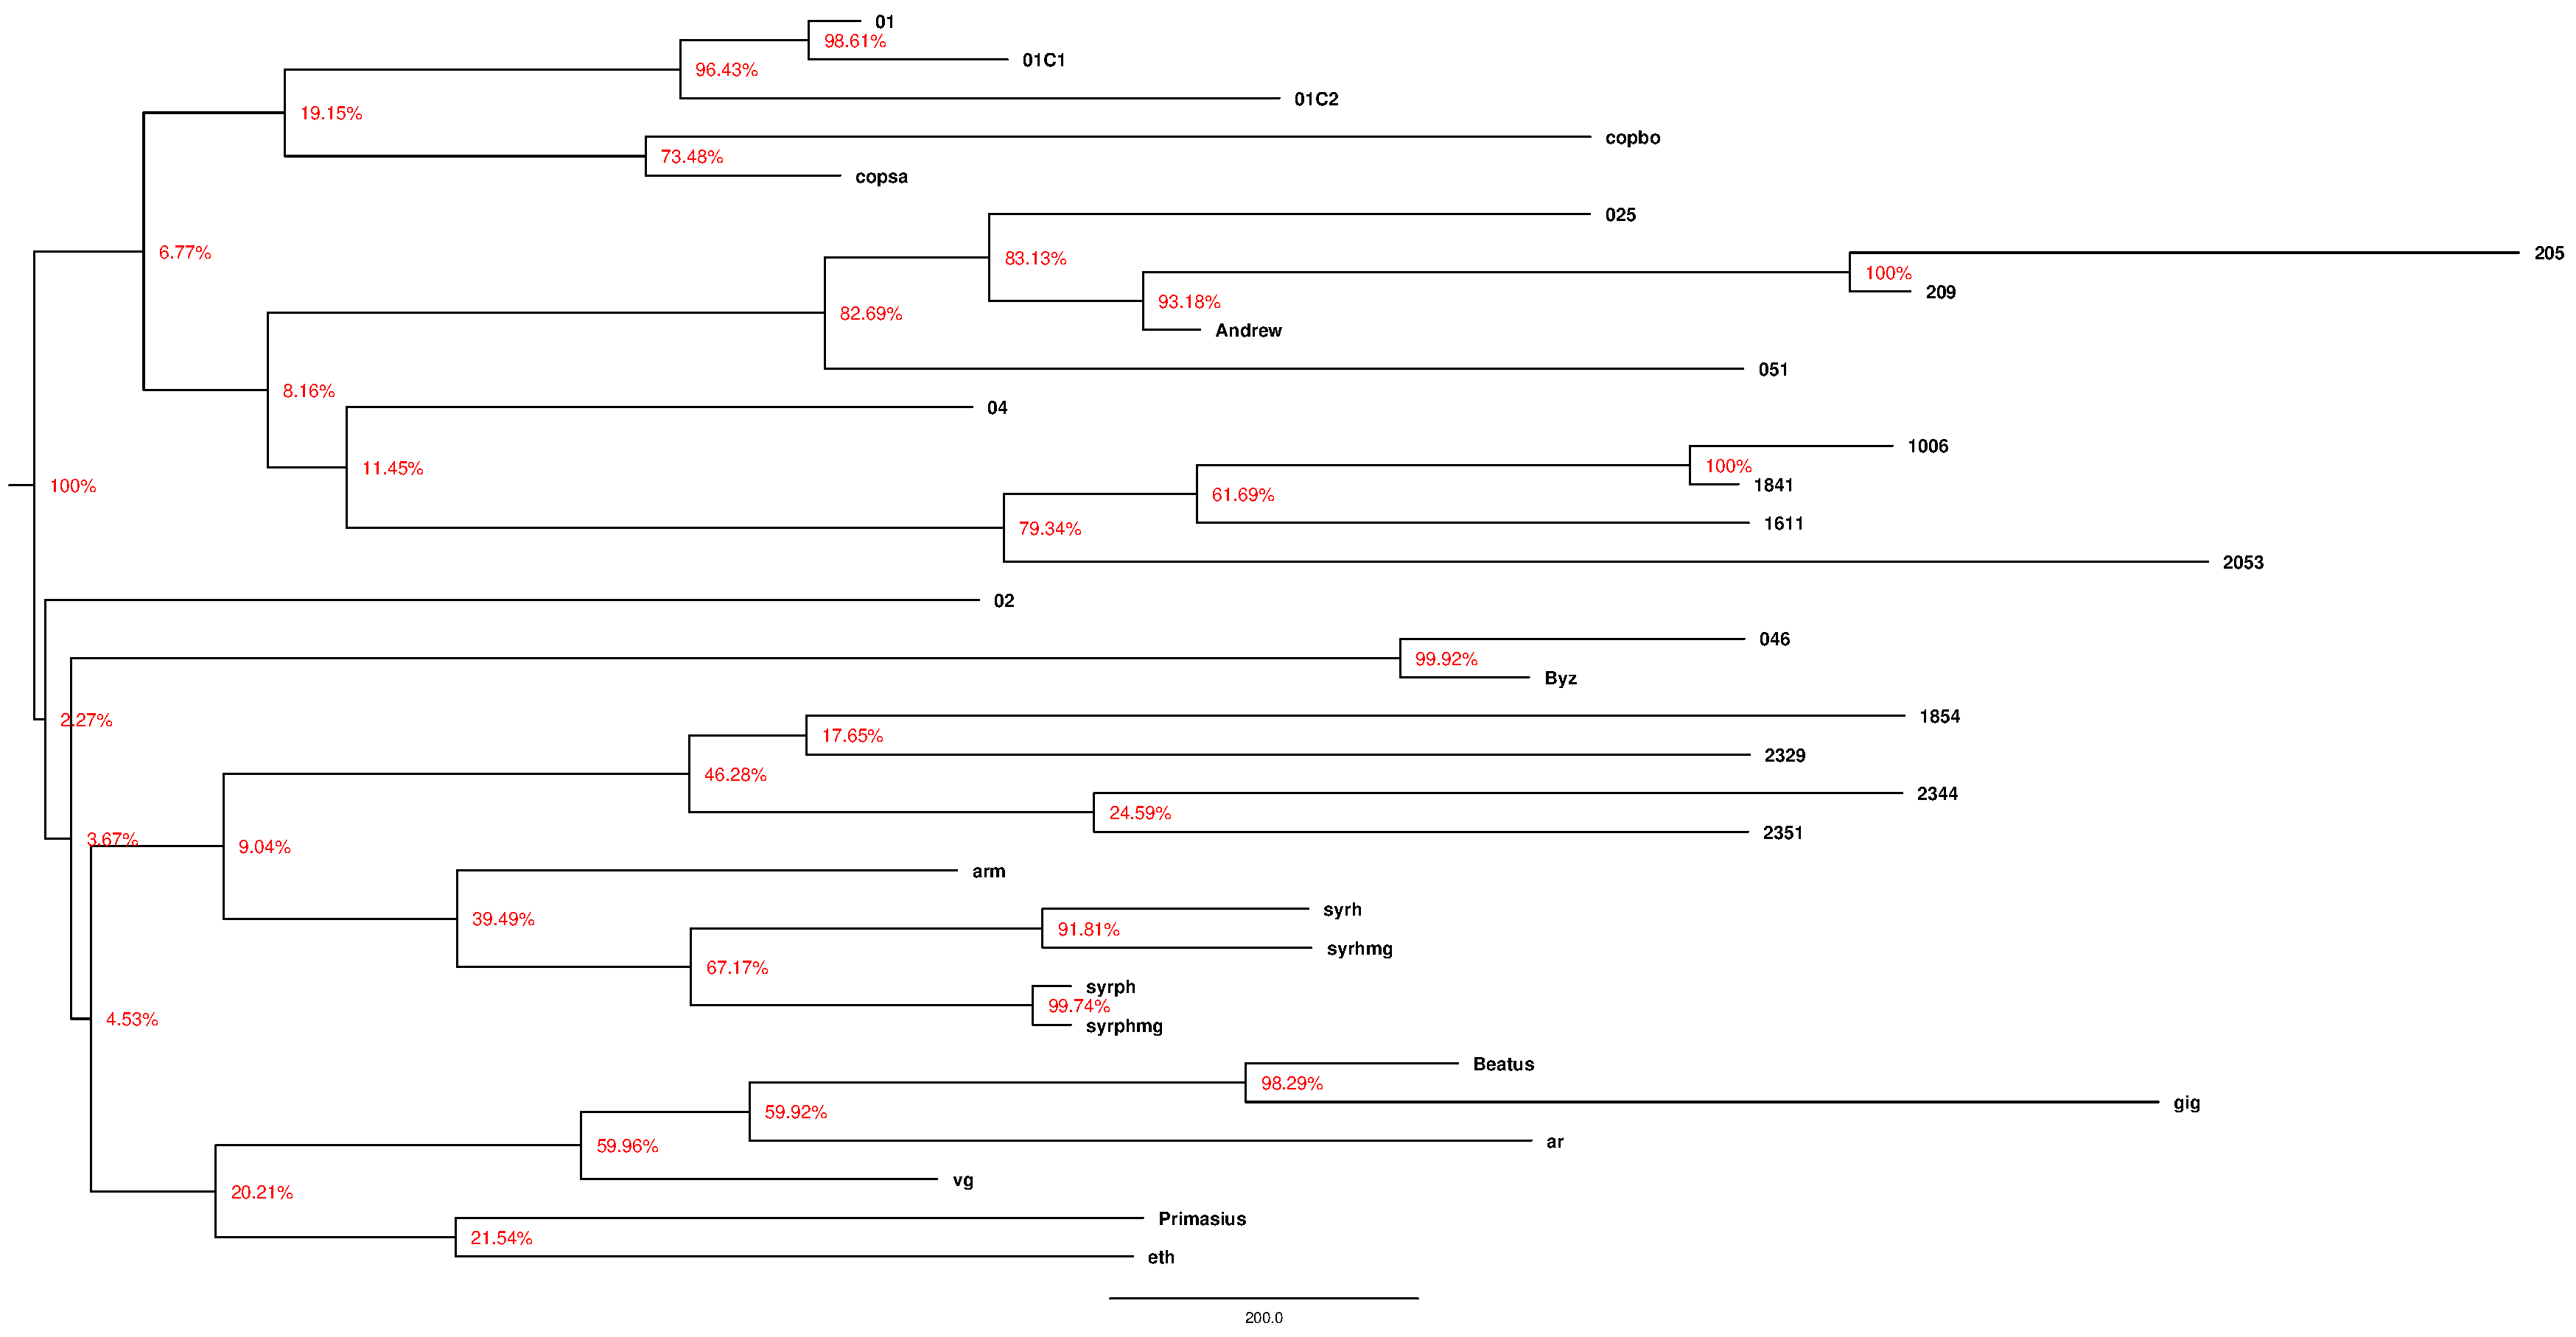
\includegraphics[width=\textwidth]{../img/ubs_revelation_local_max_clade_credibility_tree.pdf}\\
			Maximum clade credibility tree for subset of UBS Revelation data at UBS variation units (33 witnesses, 70 variation units, 20,000,000 iterations) with local clock model\\
		\end{center}
	\end{frame}
	\subsection{Mark}
	\begin{frame}
		\begin{center}
			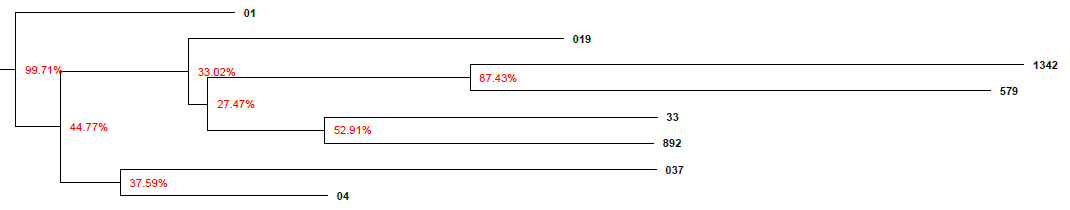
\includegraphics[width=\textwidth]{../img/ecm_mark_local_max_clade_credibility_tree_a_text.png}\\
			Subset of maximum clade credibility tree for ECM Mark data at UBS variation units (167 witnesses, 148 variation units, 20,000,000 iterations) with local clock model\\
		\end{center}
	\end{frame}
	\begin{frame}
		\begin{center}
			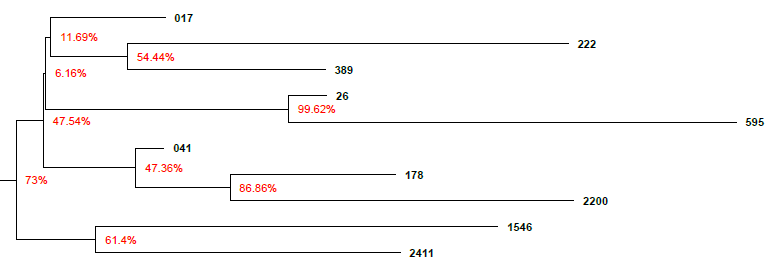
\includegraphics[width=\textwidth]{../img/ecm_mark_local_max_clade_credibility_tree_family_041.png}\\
			Subset of maximum clade credibility tree for ECM Mark data at UBS variation units (167 witnesses, 148 variation units, 20,000,000 iterations) with local clock model\\
		\end{center}
	\end{frame}
	\begin{frame}
		\begin{center}
			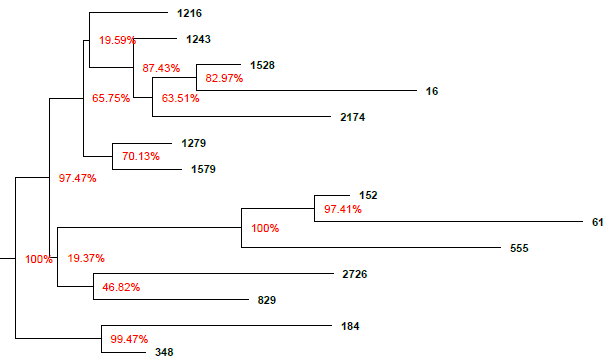
\includegraphics[width=\textwidth]{../img/ecm_mark_local_max_clade_credibility_tree_family_1216.png}\\
			Subset of maximum clade credibility tree for ECM Mark data at UBS variation units (167 witnesses, 148 variation units, 20,000,000 iterations) with local clock model\\
		\end{center}
	\end{frame}
	\begin{frame}
		\begin{center}
			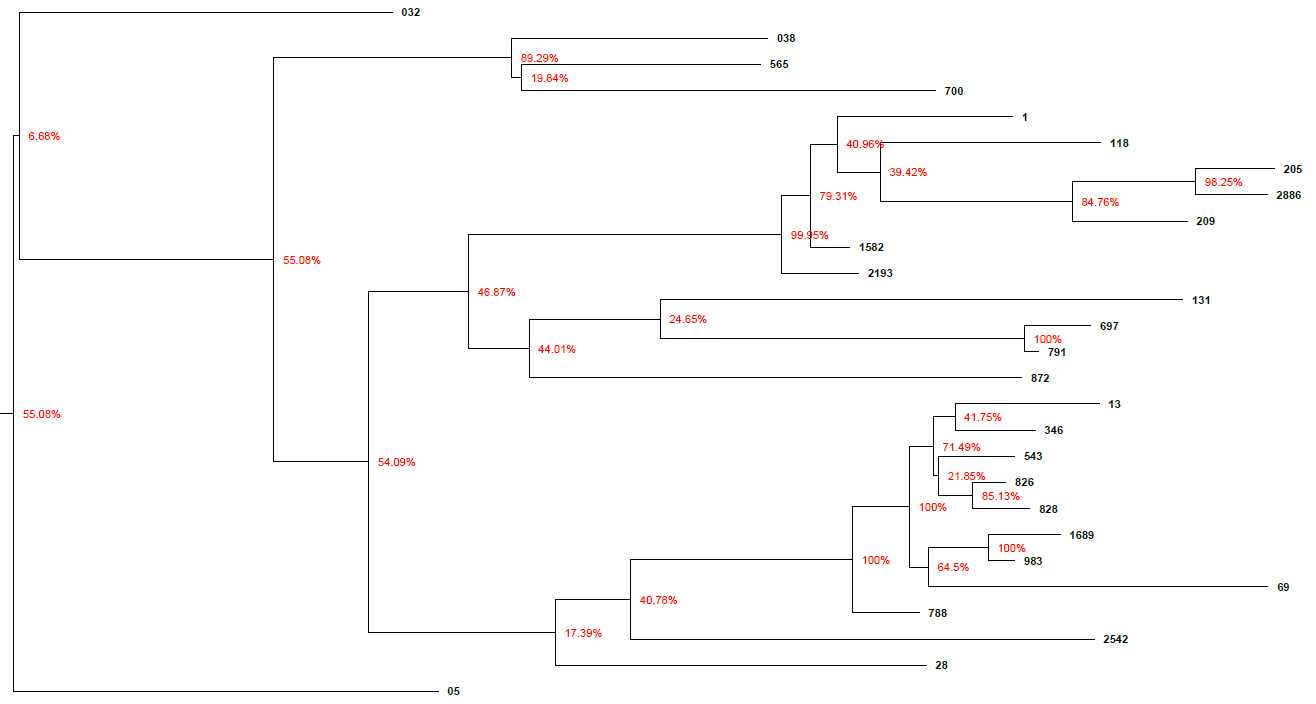
\includegraphics[width=\textwidth]{../img/ecm_mark_local_max_clade_credibility_tree_caesarean.png}\\
			Subset of maximum clade credibility tree for ECM Mark data at UBS variation units (167 witnesses, 148 variation units, 20,000,000 iterations) with local clock model\\
		\end{center}
	\end{frame}
	\begin{frame}
		\begin{center}
			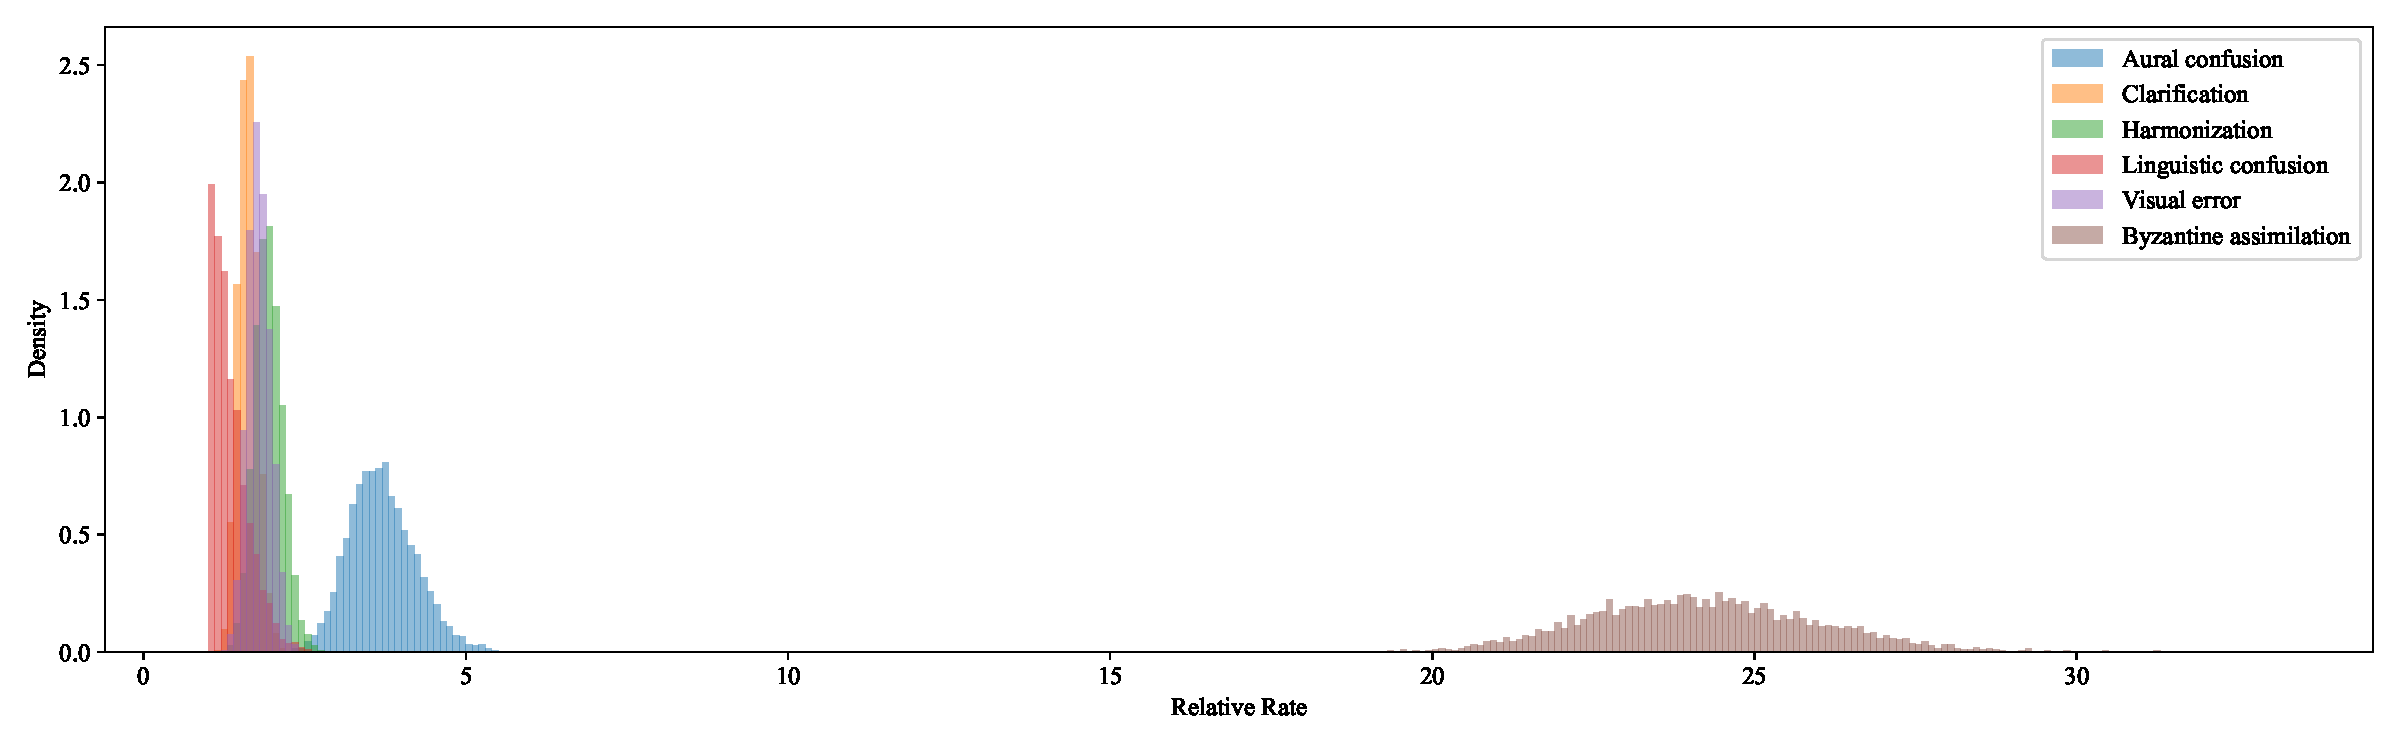
\includegraphics[width=\textwidth]{../img/ecm_mark_local_rates.pdf}\\
			Transcriptional rate posteriors for ECM Mark data at UBS variation units (167 witnesses, 148 variation units, 20,000,000 iterations) with local clock model\\
		\end{center}
	\end{frame}
		\subsection{Ephesians}
	\begin{frame}
		\begin{center}
			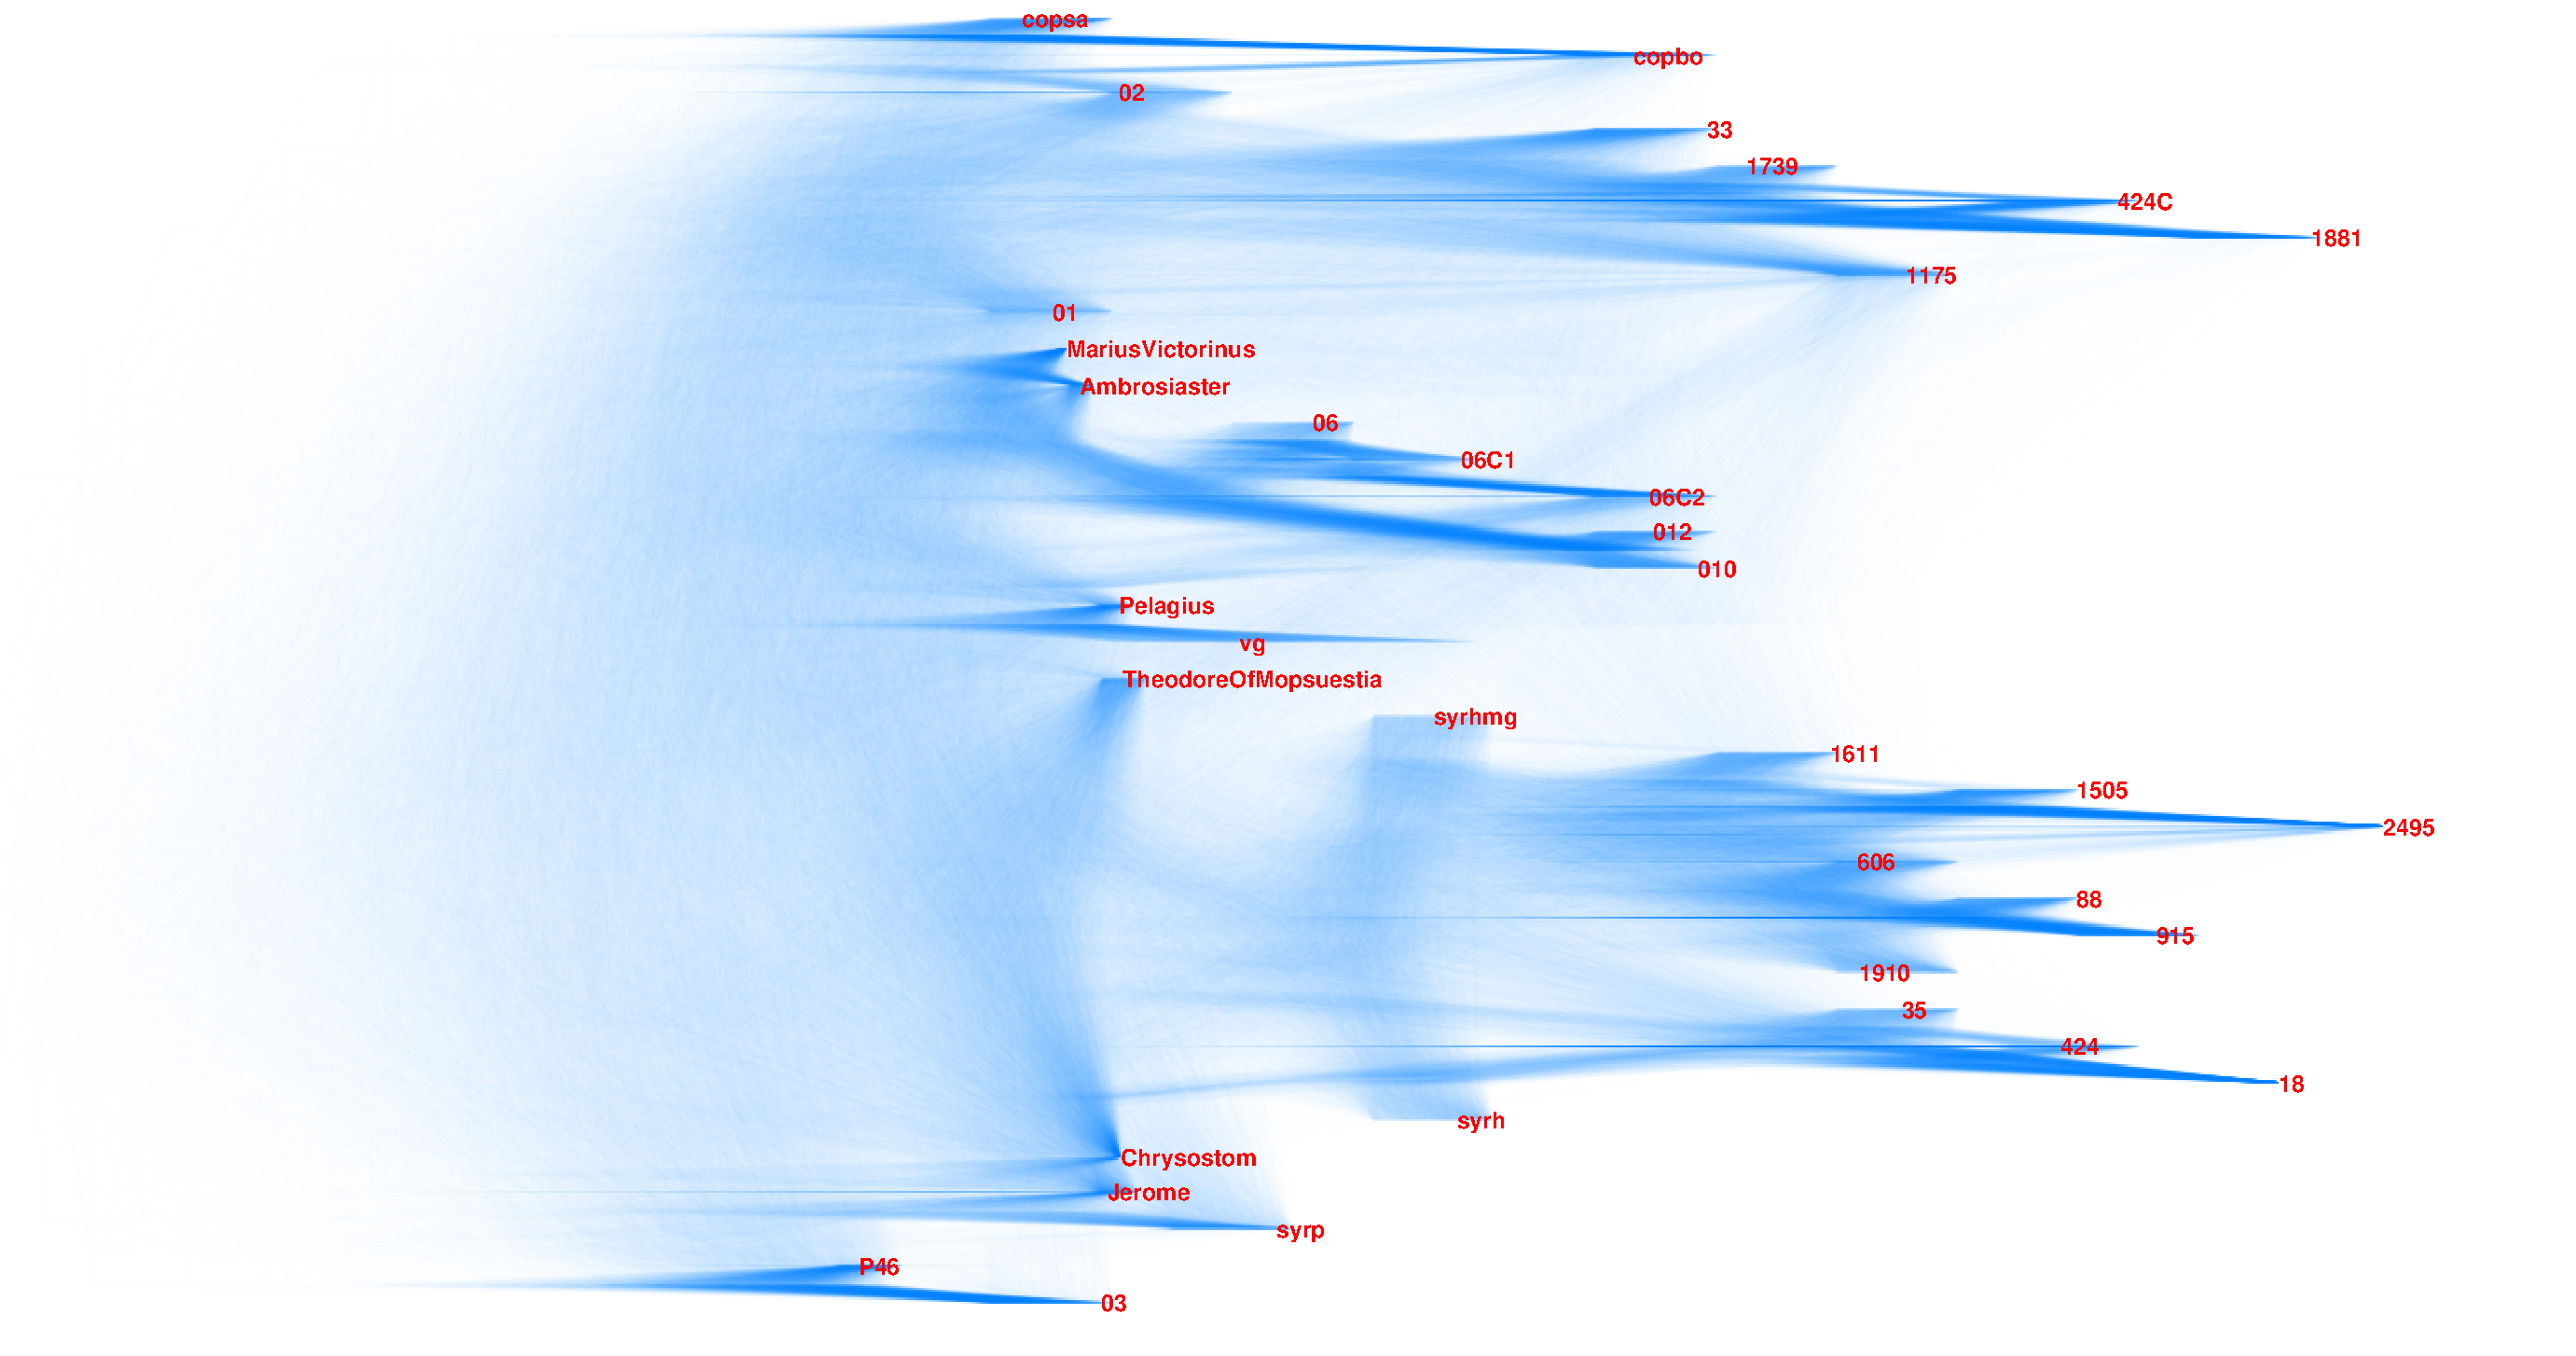
\includegraphics[width=\textwidth]{../img/ubs_ephesians_local_densitree.pdf}\\
			Posterior distribution of stemmata for subset of UBS Ephesians data at UBS variation units (36 witnesses, 42 variation units, 20,000,000 iterations) with local clock model\\
		\end{center}
	\end{frame}
	\begin{frame}
		\begin{center}
			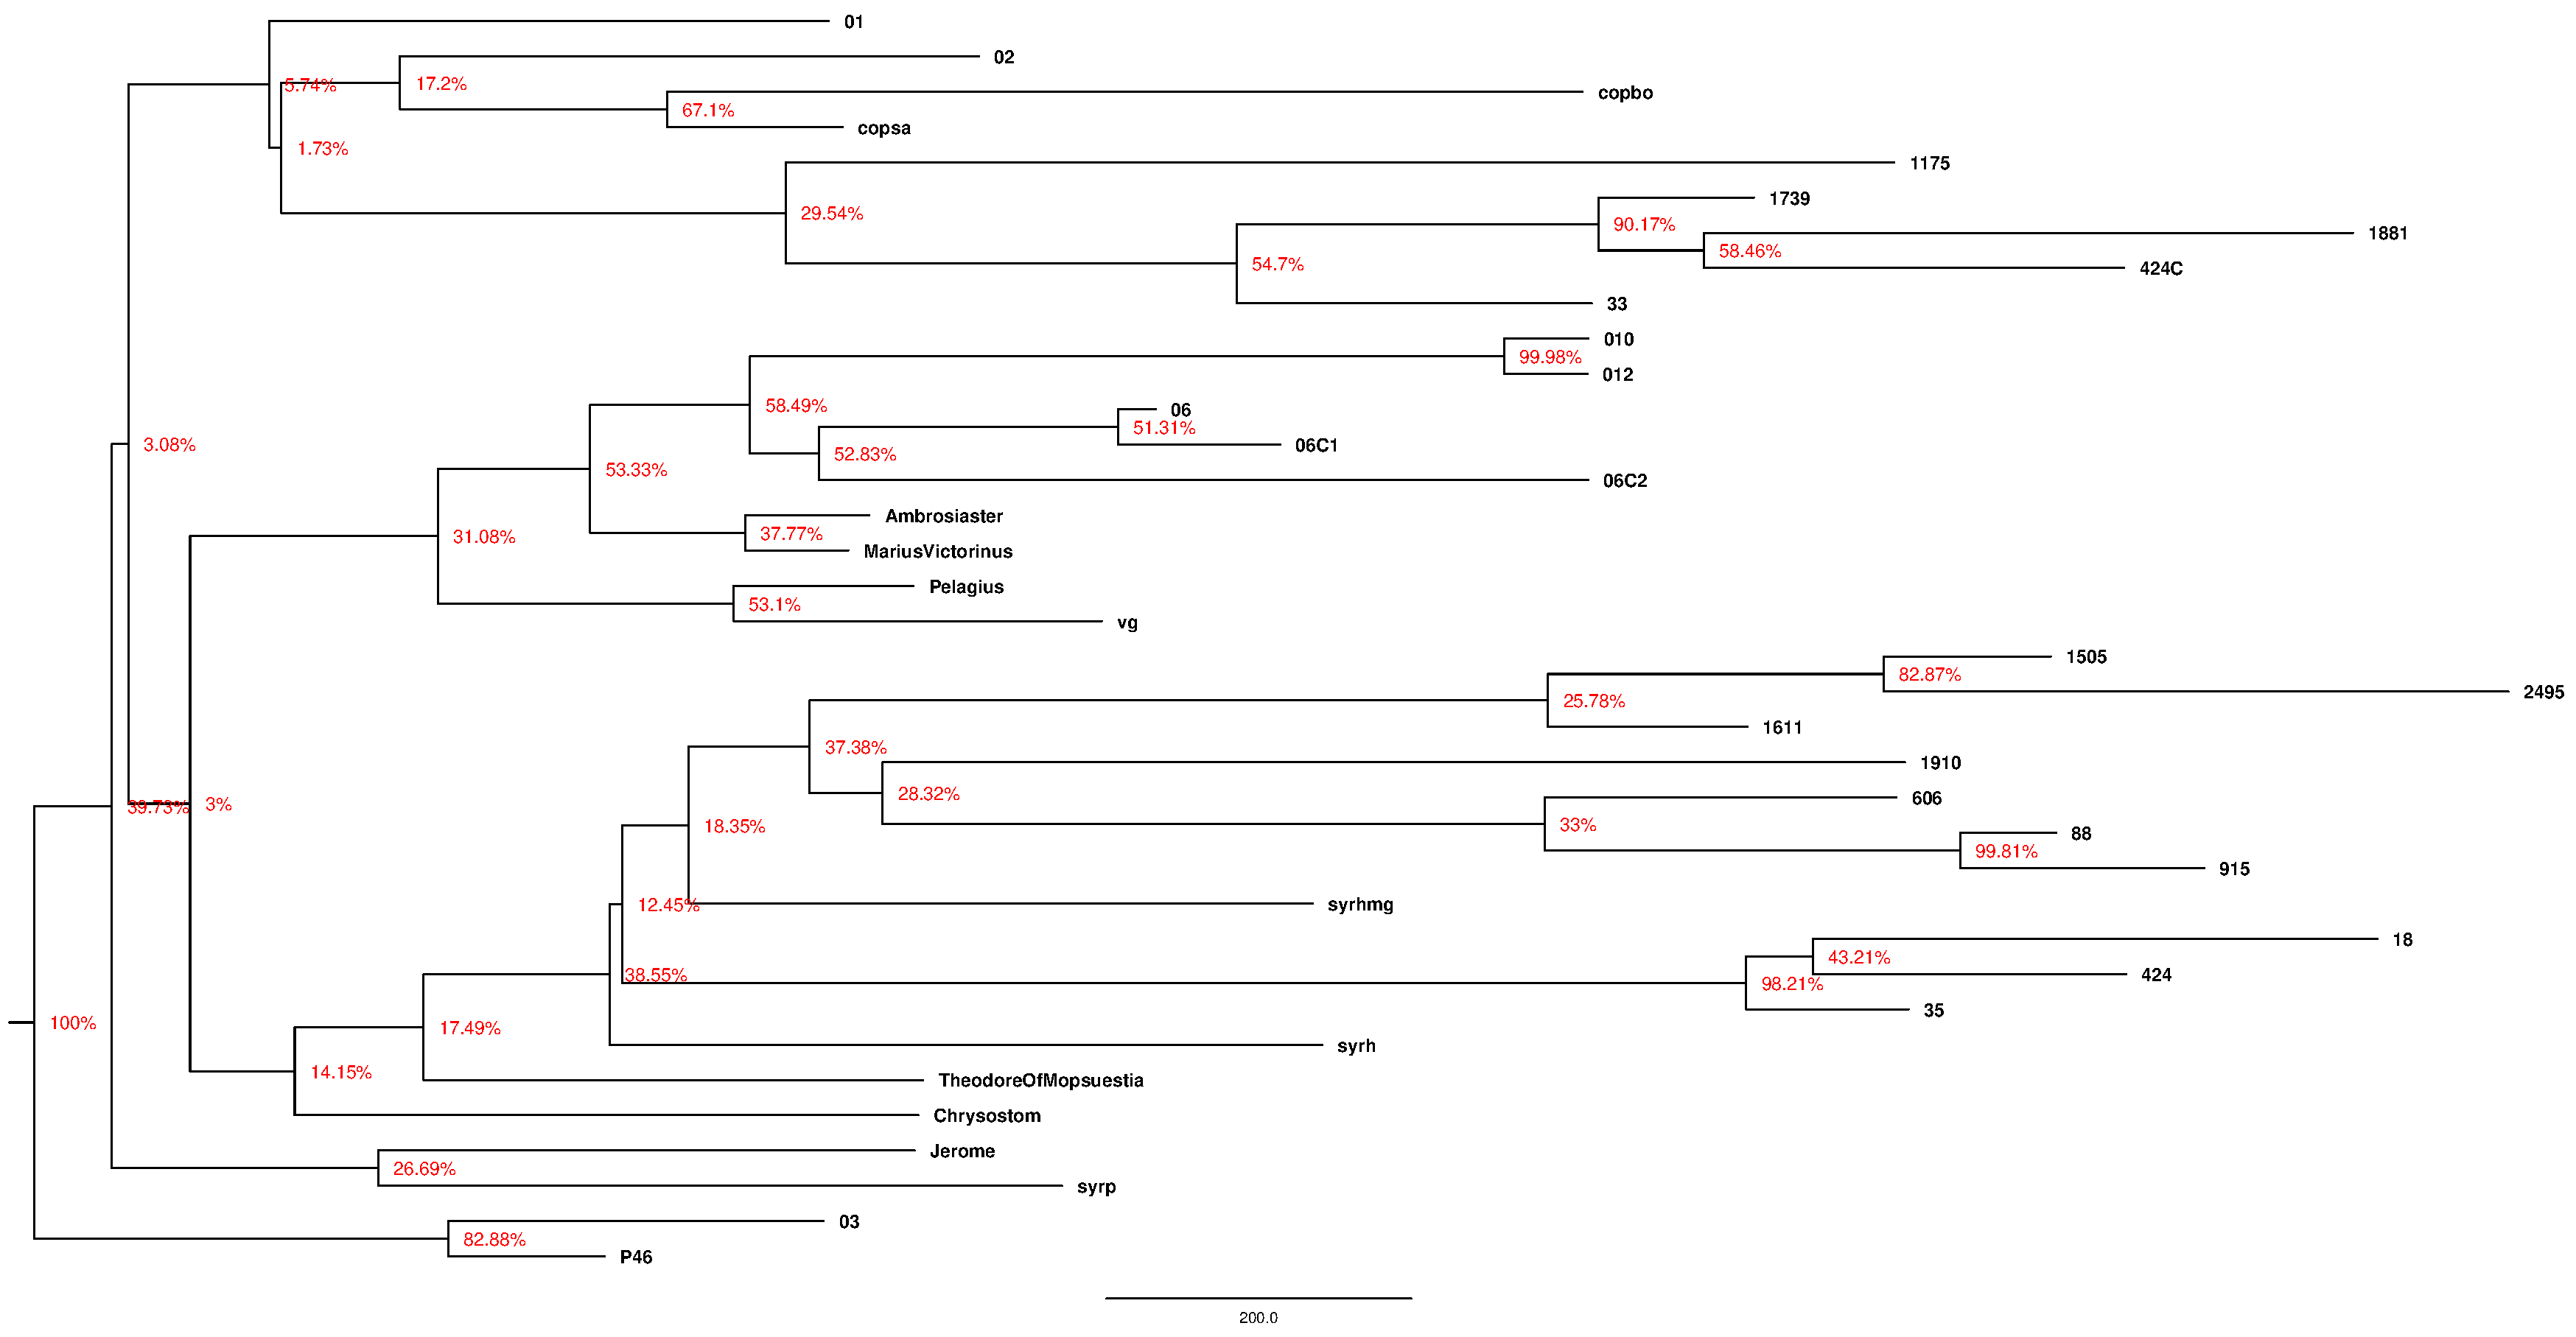
\includegraphics[width=\textwidth]{../img/ubs_ephesians_local_max_clade_credibility_tree.pdf}\\
			Maximum clade credibility tree for subset of UBS Ephesians data at UBS variation units (36 witnesses, 42 variation units, 20,000,000 iterations) with local clock model\\
		\end{center}
	\end{frame}
	\begin{frame}
		\begin{center}
			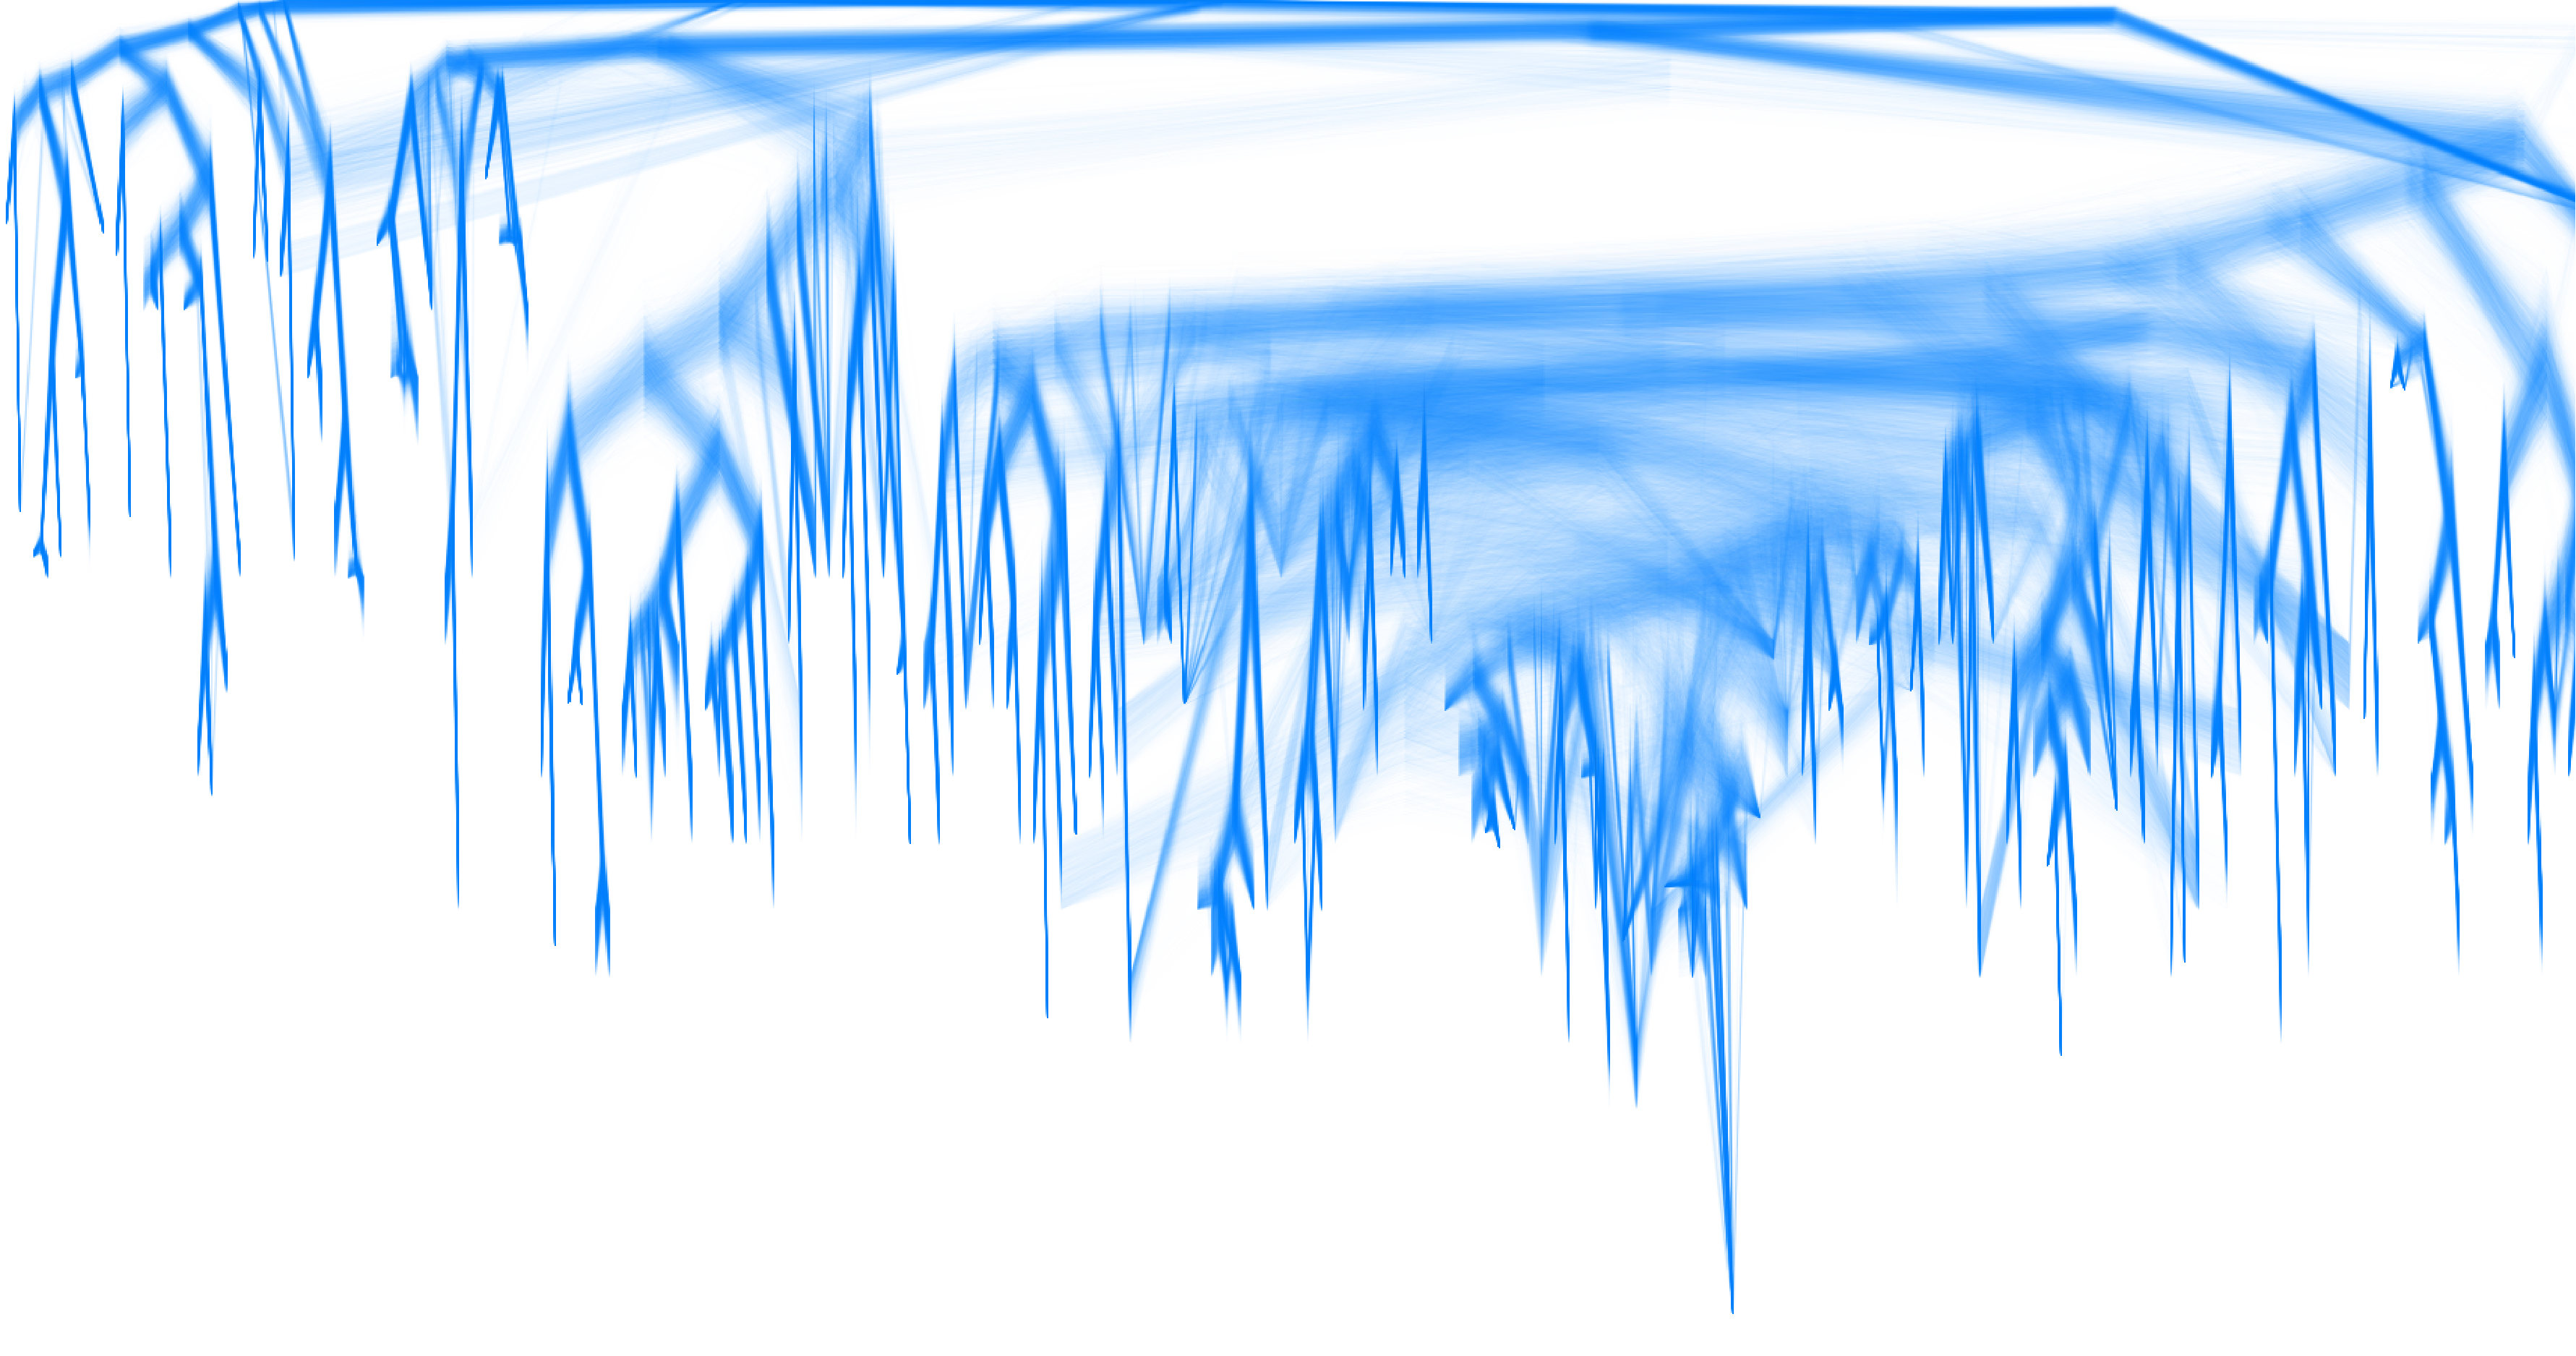
\includegraphics[width=\textwidth]{../img/igntp_ephesians_strict_densitree_unlabeled.pdf}\\
			Posterior distribution of stemmata for IGNTP Ephesians data at all variation units (193 witnesses, 915 variation units, 20,000,000 iterations) with strict clock model\\
			(Details to come later!)
		\end{center}
	\end{frame}
	\section{Conclusion}
	\begin{frame}
		For more details:
		\begin{itemize}
			\item Joey McCollum and Robert Turnbull, \textquote{\texttt{teiphy}: A Python Package for Converting TEI XML to NEXUS and Other Formats}, \emph{Journal of Open Source Software} 7.80 (2022): 4879, \textsc{doi}:\href{https://doi.org/10.21105/joss.04879}{10.21105/joss.04879}
			\item Joey McCollum and Robert Turnbull, \textquote{Using Bayesian Phylogenetics to Infer Manuscript Transmission History} (submitted, in revision)
			\item Joey McCollum, \textquote{Bayesian Stemmatology and Its Application to the Text of Ephesians} (PhD diss., Australian Catholic University, expected 2025)
			\item The datasets and outputs for this presentation are freely available at \url{https://github.com/jjmccollum/sbl-2023-talk}
		\end{itemize}
	\end{frame}
\end{document}